\documentclass[a4,10pt]{article} \usepackage[pdftex]{graphicx}
\usepackage{setspace}
%\usepackage{lineno}
\usepackage{color}
\usepackage{hyperref}
\hypersetup{
    colorlinks,%
    citecolor=black,%
    filecolor=black,%
    linkcolor=black,%
    urlcolor=blue
}
\definecolor{PiranaOrange}{rgb}{0.9,0.4,0.1}
\definecolor{Blue}{rgb}{0.0,0.0,0.7}
\definecolor{Red}{rgb}{0.7,0.0,0.0}
\definecolor{Grey}{rgb}{0.2,0.2,0.2}
\definecolor{grey2}{rgb}{.92, .92, .92}

\pdfinfo{
   /Author (Ron Keizer, Coen van Hasselt, Pirana Software & Consulting BV)
   /Title  (Pirana Quick Guide)
}


\bibliographystyle{unsrt}%Choose a bibliograhpic style}
%\usepackage{utopia} %\usepackage{charter} %\usepackage{palatino}
%\usepackage{bookman} %\usepackage{newcent} %\usepackage{times}
%\usepackage[options]{natbib} \sloppy
\renewcommand{\familydefault}{\sfdefault} 
\renewcommand{\emph}[1]{\textbf{\textcolor{Grey}{#1}}} 
\oddsidemargin 1cm
\textwidth 14cm
\textheight 20cm

\begin{document}

{\centering
  \vspace{-100pt}
  \textbf{
    \textcolor{PiranaOrange}{\Large Pirana}
  }\\
  \vspace{5pt} \scriptsize \textcolor{Grey}{The flexible modeling
    environment for NONMEM} \\ \normalsize
  \vspace{12pt}
  \hspace{5pt}
\includegraphics[scale=0.14]{images/pirana_logo.jpg}\\
  \vspace{18pt}

  {\large
    \emph{Quick Guide: Using PsN from Pirana}  \vspace{10pt} \\
        Version 1.1
  }

}
\vspace{25pt}

\begin{center}
   {\colorbox{grey2}{
         \begin{minipage}[t]{0.9\textwidth}
\subsubsection*{Scope}
This Pirana Quick Guide explains how to use Pirana to work with the
modeling toolkit Perl speaks NONMEM (PsN). This freely available
toolkit is developed by Uppsala University and extends the
funtionality of NONMEM with many tools, e.g. for advanced execution of
models, performing bootstraps of model estimations, stepwise covariate
modeling, log-likelihood profiling, stochastic simulation and
(re-)estimation, and many more. PsN can also be used to generate
various diagnostics, such as visual and numeric predictive checks (VPC
/ NPC). \\

\textit{Note: this is not a guide to PsN itself. If you have questions
  on the use of PsN, please check the PsN manual or contact the
  developers of PsN at http://psn.sourceforge.net.}
          \end{minipage}
      }
   }
\end{center}

\subsubsection*{Introduction / Setting up PsN}
\begin{itemize}
\item  If you haven't installed PsN, download the latest
  version from http://psn.sourceforge.net, and follow the
  instructions.
\item The most important part after installation is to make
  sure that PsN knows where NONMEM is installed. PsN can do this for
 you automatically during the installation.
\item To configure NONMEM installations manually for PsN,
 look up the file \textbf{psn.conf} in the folder where PsN
  was installed (on Windows probably somewhere in
  C:$\backslash$Perl$\backslash$site$\backslash$PsN\_x\_x\_x. (Note
  that an alternative psn.conf can be created in your home folder
  which overrides the system-wide psn.conf.) Open the configuration
  file in a text editor (e.g. notepad), and scroll to the section
  \textbf{[nm\_versions]}, an example is shown  in Figure \ref{fig:Fig1}

\begin{figure}[h] \centering
  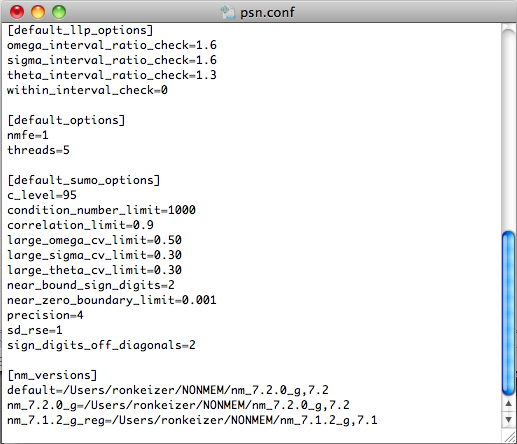
\includegraphics[scale=.4]{images/psn_conf.png}
  \caption{Edit PsN configuration file\label{fig:Fig1}}
\end{figure}

\item In this \textbf{[nm\_versions]} section you should define where
  NONMEM versions are installed on your system, and which
  version. Follow the comments and examples that are given in the PsN
  website if you are not sure what to put here.

\end{itemize}

\subsubsection*{Using the execute command}

\begin{itemize}
\item First, we will show how the PsN \textit{execute} command can be used
from Pirana. 

\item Select a model that you want to run in NONMEM, right-click with
  the mouse in the model overview, and select \textbf{PsN
    $\rightarrow$ execute}. This will bring up the PsN dialog for this
  command. Alternatively, you can use the Ctrl-E shortcut to do
  this. Now you will see the following window:

\begin{figure}[h] \centering
  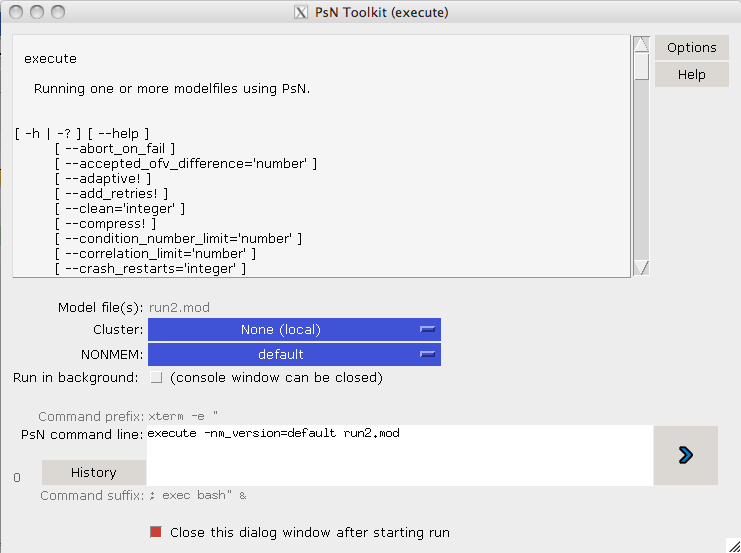
\includegraphics[scale=.4]{images/psn_dialog.png}
  \caption{The PsN dialog in Pirana\label{fig:Fig2}}
\end{figure}

\item The top part of this window shows the help file for this command. On
the right-hand side you can choose whether you want to see the short
help file only a list of the available arguments, or a long help file
with explanations of the various arguments. 

\item In the text-box below, the actual PsN command can be typed. This will
look something like:

\begin{verbatim}
execute -nm_version=default run1.mod
\end{verbatim}

\item To this command you can add arguments that you require. Many options
are available, it is highly recommended to look into the available
options. But for now let's just start the command like this. Pres the
run button (>), and Pirana will start the execute command, as shown in
the screenshot below.

\begin{figure}[h] \centering
  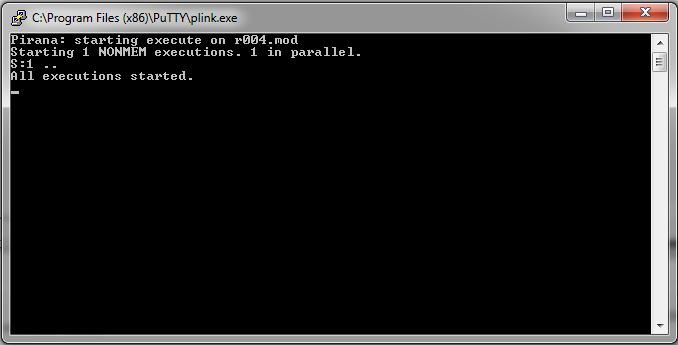
\includegraphics[scale=.4]{images/psn_run.png}
  \caption{A PsN run in Windows (but run on a Linux cluster)\label{fig:Fig3} }
\end{figure}

\item What PsN actually does is create a subfolder in which the run is
executed. After the NONMEM run finishes, PsN will copy back the
results files to the main folder.
\item Note that Pirana does not automatically detect that new results
  are available, so you should press the refresh button to load the
  results into the Pirana overview. To show the folders that PsN has
  created in the main overview, you have to select either `PsN
  folders' or `All folders' from the folder selection menu,
  highlighted below.
\end{itemize}

\subsubsection*{Using the other PsN tools}
The other PsN tools are used in exactly the same way. For example to
start a bootstrap, select a model and select `bootstrap' from the PsN
menu (under `Model evaluation'), or using the Ctrl-B shortcut. Make
sure that at least the {\ttfamily -samples=...} argument is present in
the command to be executed.

\begin{itemize}
\item You will notice that a `History' button is present in the dialog as
well. From the command list that is opened by clicking this button,
you can select previously used PsN commands. Alternatively from the
main PsN dialog you can also retrieve previously executed command by
using Ctrl-up and Ctrl-down buttons.

\item If there are special argument that you commonly use, you can set
  them as defaults. In Pirana, go to \textbf{Settings $\rightarrow$
    PsN}. As shown in Figure \ref{fig:Fig2} you can set here the default
  arguments for all PsN commands.

\end{itemize}
\begin{figure}[h] \centering
  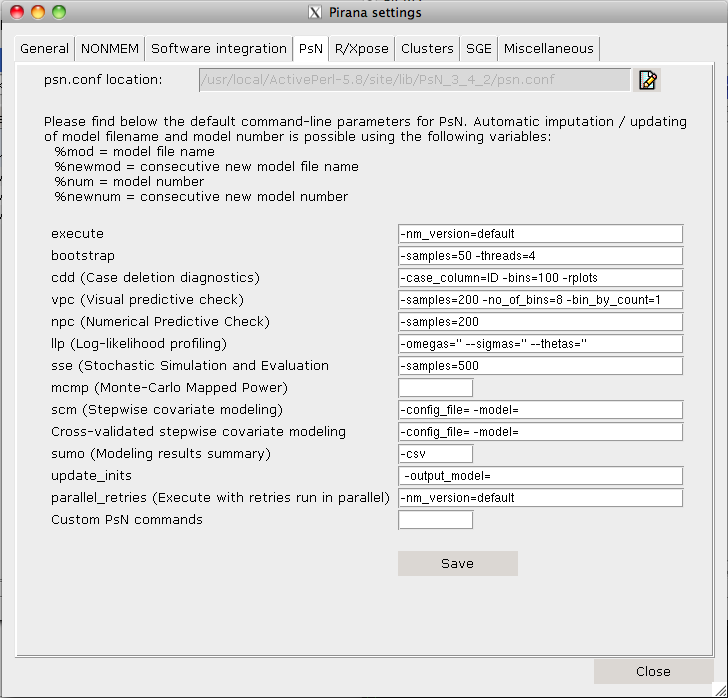
\includegraphics[scale=.4]{images/psn_defaults.png}
  \caption{PsN default arguments in Pirana\label{fig:Fig4}}
\end{figure}

\subsubsection*{Using PsN data transformation tools}
Besides tools for working with NONMEM executions, PsN also
incorporates some tools to format or transform datasets, or display
some statistics. To use these tools, go the file list on the right
side of the Pirana window. Select a table or csv-file, and right
click. From the menu select e.g. \textbf{PsN $\rightarrow$ data\_stats}.

\begin{itemize}
\item A dialog window will now open, similar to the other PsN tools. You
will notice that the \textbf{data\_stats} tool only takes a few
arguments. 

\begin{figure}[h] \centering
  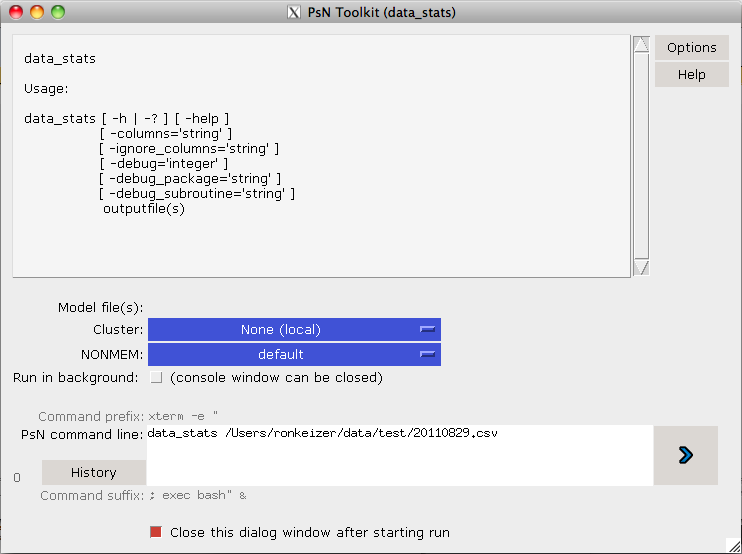
\includegraphics[scale=.4]{images/psn_data_stats.png}
  \caption{The PsN data\_stats dialog in Pirana\label{fig:Fig5}}
\end{figure}

\item If you run this on a csv-file, In the console window that will be
opened, some statistics are printed for each column in the dataset.

\item The other PsN dataset tools work in exactly the same way, although
they perform conversions rather than printing information only.
\end{itemize}


\end{document}
